\chapter{Preliminaries}

\section{Linear Algebra}

\subsection{Vectors and Matrices}

\subsubsection{Operations with Matrices}

Let \(A = (a_{ij})\) and \(B = (b_{ij})\) be matrices in \(\mathbb{K}^{m \times n}\), where \(\mathbb{K}\) is a field (e.g., \(\mathbb{R}\) or \(\mathbb{C}\)). We say \(A = B\) if and only if \(a_{ij} = b_{ij}\) for all \(i = 1,\ldots,m\) and \(j = 1,\ldots,n\).

\begin{definition}{Matrix Addition and Scalar Multiplication}{matrix-add-scalar}

    \begin{itemize}[nosep]
        \item \textbf{Matrix sum:} \((A+B)_{ij} = a_{ij} + b_{ij}\) for all \(i,j\). The additive identity is the \emph{zero matrix} \(0\), with all entries zero.
        \item \textbf{Scalar multiplication:} For \(\lambda \in \mathbb{K}\), \((\lambda A)_{ij} = \lambda a_{ij}\).
    \end{itemize}

\end{definition}

\begin{example}{Matrix Addition and Scalar Multiplication}{}
    Let \(A = \begin{pmatrix}1 & 2\\3 & 4\end{pmatrix}\), \(B = \begin{pmatrix}5 & 6\\7 & 8\end{pmatrix}\), and \(\lambda = 2\).
    \[
        A+B = \begin{pmatrix}1+5 & 2+6\\3+7 & 4+8\end{pmatrix} = \begin{pmatrix}6 & 8\\10 & 12\end{pmatrix},\quad
        2A =
        \begin{pmatrix}
            2\cdot1 & 2\cdot2 \\
            2\cdot3 & 2\cdot4
        \end{pmatrix}
        =
        \begin{pmatrix}
            2 & 4 \\
            6 & 8
        \end{pmatrix}
    \]
\end{example}

\begin{definition}{Matrix Multiplication}{matrix-mult}
    Let \(A \in \mathbb{K}^{m \times p}\) and \(B \in \mathbb{K}^{p \times n}\). The \emph{matrix product} \(C = AB \in \mathbb{K}^{m \times n}\) is defined by
    \[
        c_{ij} = \sum_{k=1}^p a_{ik} b_{kj}, \quad \text{for } i=1,\ldots,m,\ j=1,\ldots,n.
    \]
\end{definition}

\begin{example}{Matrix Multiplication}{}
    Let \(A = \begin{pmatrix}1 & 2\\3 & 4\end{pmatrix}\), \(B = \begin{pmatrix}0 & 1\\1 & 0\end{pmatrix}\).
    \[
        AB = \begin{pmatrix}
            1\cdot0 + 2\cdot1 & 1\cdot1 + 2\cdot0 \\
            3\cdot0 + 4\cdot1 & 3\cdot1 + 4\cdot0
        \end{pmatrix}
        = \begin{pmatrix}2 & 1\\4 & 3\end{pmatrix}
    \]
\end{example}

\begin{property}{Matrix Operations}{matrix-properties}
    \begin{itemize}[nosep]
        \item Matrix addition is commutative and associative.
        \item Matrix multiplication is associative and distributive over addition, but \textbf{not} commutative in general: \(AB \neq BA\).
        \item The \emph{identity matrix} \(I_n = (\delta_{ij})\) (where \(\delta_{ij}\) is the Kronecker delta) satisfies \(AI_n = I_nA = A\) for all \(A \in \mathbb{K}^{n \times n}\).
        \item A \emph{diagonal matrix} is \(D = \operatorname{diag}(d_1,\ldots,d_n)\), i.e., \(D_{ij} = d_i\) if \(i=j\), \(0\) otherwise.
        \item For \(A \in \mathbb{K}^{n \times n}\) and \(p \in \mathbb{N}\), \(A^p\) denotes the \(p\)-fold product of \(A\) with itself, with \(A^0 = I_n\).
    \end{itemize}
\end{property}

\begin{figure}[H]
    \centering
    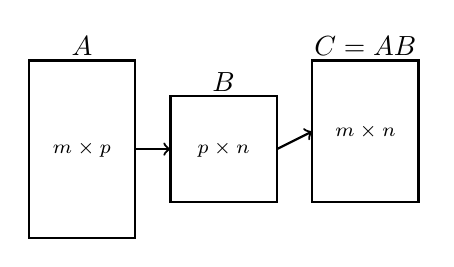
\begin{tikzpicture}[scale=0.9]
        % A: m x p
        \draw[thick] (0,0) rectangle (1.5,2.5);
        \node at (0.75,2.7) {\(A\)};
        \node at (0.75,1.25) {\scriptsize \(m \times p\)};
        % B: p x n
        \draw[thick] (2,0.5) rectangle (3.5,2);
        \node at (2.75,2.2) {\(B\)};
        \node at (2.75,1.25) {\scriptsize \(p \times n\)};
        % C: m x n
        \draw[thick] (4,0.5) rectangle (5.5,2.5);
        \node at (4.75,2.7) {\(C=AB\)};
        \node at (4.75,1.5) {\scriptsize \(m \times n\)};
        % Arrows
        \draw[->,thick] (1.5,1.25) -- (2,1.25);
        \draw[->,thick] (3.5,1.25) -- (4,1.5);
    \end{tikzpicture}
    \caption{Matrix multiplication: \(A\) (\(m \times p\)) times \(B\) (\(p \times n\)) yields \(C\) (\(m \times n\)).}
\end{figure}

\begin{remark}{Commutativity and Special Matrices}{commutativity}
    Square matrices \(A,B \in \mathbb{K}^{n \times n}\) are called \emph{commutative} if \(AB = BA\). In general, matrix multiplication is not commutative.
\end{remark}

\subsubsection{Elementary Row Operations and Matrices}

Elementary row operations on \(A \in \mathbb{K}^{m \times n}\) can be represented as multiplication by special matrices on the left:

\begin{itemize}[nosep]
    \item \textbf{Scaling row \(i\) by \(\alpha \neq 0\):} Pre-multiply by \(D = \operatorname{diag}(1,\ldots,1,\alpha,1,\ldots,1)\), where \(\alpha\) is in the \(i\)-th position.
    \item \textbf{Swapping rows \(i\) and \(j\):} Pre-multiply by the \emph{elementary permutation matrix} \(P_{(i,j)}\), which is the identity with rows \(i\) and \(j\) swapped.
    \item \textbf{Adding \(\alpha\) times row \(j\) to row \(i\):} Pre-multiply by \(E = I + \alpha E_{ij}\), where \(E_{ij}\) is the matrix with \(1\) in position \((i,j)\) and \(0\) elsewhere.
\end{itemize}

\begin{example}{Permutation Matrix}
    For \(n=3\), swapping rows \(1\) and \(2\):
    \[
        P_{(1,2)} = \begin{pmatrix}
            0 & 1 & 0 \\
            1 & 0 & 0 \\
            0 & 0 & 1
        \end{pmatrix}
    \]
\end{example}

\subsubsection{Special Types of Matrices}

\begin{definition}{Special Matrices}{special-matrices}
    Let \(A \in \mathbb{R}^{n \times n}\) or \(\mathbb{C}^{n \times n}\).
    \begin{description}[nosep]
        \item[Identity matrix:] \(I_n = (\delta_{ij})\), where \(\delta_{ij}\) is the Kronecker delta.
        \item[Diagonal matrix:] \(D = \operatorname{diag}(d_1,\ldots,d_n)\), all off-diagonal entries are zero.
        \item[Symmetric:] \(A = A^\top\).
        \item[Antisymmetric (skew-symmetric):] \(A = -A^\top\).
        \item[Orthogonal:] \(A^\top A = AA^\top = I_n\) (so \(A^{-1} = A^\top\)).
        \item[Permutation matrix:] obtained by permuting the rows of \(I_n\).
        \item[Hermitian:] \(A = A^H\), where \(A^H = \overline{A}^\top\).
        \item[Unitary:] \(A^H A = A A^H = I_n\) (so \(A^{-1} = A^H\)).
        \item[Normal:] \(A^H A = A A^H\) (complex) or \(A^\top A = A A^\top\) (real matrices).
    \end{description}
\end{definition}

\begin{example}{Orthogonal and Unitary Matrices}{}
    \begin{itemize}[nosep]
        \item \(Q = \begin{pmatrix} 0 & 1\\-1 & 0\end{pmatrix}\) is orthogonal: \(Q^\top Q = I\).
        \item \(U = \frac{1}{\sqrt{2}}\begin{pmatrix}1 & i\\i & 1\end{pmatrix}\) is unitary: \(U^H U = I\).
    \end{itemize}
\end{example}

\subsection{Matrix Inverse and Transpose}

\begin{definition}{Inverse of a Matrix}{matrix-inverse}
    A square matrix \(A \in \mathbb{K}^{n \times n}\) is said to be \emph{invertible} (or \emph{nonsingular}) if there exists a matrix \(A^{-1} \in \mathbb{K}^{n \times n}\) such that
    \[
        AA^{-1} = A^{-1}A = I_n,
    \]
    where \(I_n\) is the \(n \times n\) identity matrix. The matrix \(A^{-1}\) is called the \emph{inverse} of \(A\).
\end{definition}

\begin{property}{Invertibility and Linear Independence}{invertible-li}
    A matrix \(A \in \mathbb{K}^{n \times n}\) is invertible if and only if its columns (or, equivalently, its rows) form a linearly independent set in \(\mathbb{K}^n\). Equivalently, \(\det(A) \neq 0\).
\end{property}

\begin{remark}{Inverse of a Product}{inverse-product}
    If \(A, B \in \mathbb{K}^{n \times n}\) are invertible, then
    \[
        (AB)^{-1} = B^{-1}A^{-1}.
    \]
    More generally, for invertible matrices \(A_1, A_2, \ldots, A_k\),
    \[
        (A_1A_2\cdots A_k)^{-1} = A_k^{-1} \cdots A_2^{-1} A_1^{-1}.
    \]
\end{remark}

\begin{definition}{Transpose and Conjugate Transpose}{transpose}
    Let \(A = (a_{ij}) \in \mathbb{K}^{m \times n}\).
    \begin{itemize}[nosep]
        \item The \emph{transpose} of \(A\) is the matrix \(A^\top \in \mathbb{K}^{n \times m}\) defined by
              \[
                  (A^\top)_{ij} = a_{ji}.
              \]
        \item If \(\mathbb{K} = \mathbb{C}\), the \emph{conjugate transpose} (or \emph{adjoint}) is \(A^H = \overline{A}^\top\), i.e.,
              \[
                  (A^H)_{ij} = \overline{a_{ji}}.
              \]
    \end{itemize}
\end{definition}

\begin{property}{Transpose Properties}{transpose-props}
    Let \(A \in \mathbb{K}^{m \times n}\), \(B \in \mathbb{K}^{n \times p}\), and \(\lambda \in \mathbb{K}\).
    \begin{itemize}[nosep]
        \item \((A^\top)^\top = A\)
        \item \((A+B)^\top = A^\top + B^\top\)
        \item \((AB)^\top = B^\top A^\top\)
        \item \((\lambda A)^\top = \lambda A^\top\)
        \item If \(A\) invertible, \((A^\top)^{-1} = (A^{-1})^\top\)
    \end{itemize}
    Analogous properties hold for \(A^H\).
\end{property}

\begin{example}{Symmetric, Skew-Symmetric, Hermitian, Unitary}{}
    \begin{itemize}[nosep]
        \item \(A = \begin{pmatrix}2 & 3\\3 & 2\end{pmatrix}\) is symmetric.
        \item \(B = \begin{pmatrix}0 & 1\\-1 & 0\end{pmatrix}\) is skew-symmetric.
        \item \(C = \begin{pmatrix}2 & i\\-i & 3\end{pmatrix}\) is Hermitian.
        \item \(U = \frac{1}{\sqrt{2}}\begin{pmatrix}1 & i\\i & 1\end{pmatrix}\) is unitary.
    \end{itemize}
\end{example}

\begin{remark}{Diagonal Entries of Hermitian Matrices}{hermitian-diag}
    If \(A\) is Hermitian, then \(a_{ii} \in \mathbb{R}\) for all \(i\).
\end{remark}

\subsubsection{Algebraic and Geometric Multiplicity}

\begin{definition}{Algebraic and Geometric Multiplicity}{alg-geom-mult}
    Let \(A \in \mathbb{C}^{n \times n}\) and \(\lambda\) be an eigenvalue of \(A\).
    \begin{itemize}[nosep]
        \item The \emph{algebraic multiplicity} of \(\lambda\), denoted \(m_a(\lambda)\), is its multiplicity as a root of the characteristic polynomial \(\det(A - \lambda I) = 0\).
        \item The \emph{geometric multiplicity} of \(\lambda\), denoted \(m_g(\lambda)\), is the dimension of the eigenspace \(\ker(A - \lambda I)\), i.e., the number of linearly independent eigenvectors associated with \(\lambda\).
        \item Always \(1 \leq m_g(\lambda) \leq m_a(\lambda)\).
    \end{itemize}
\end{definition}

\begin{example}{Algebraic vs. Geometric Multiplicity}{alg-geom-mult-ex}
    Consider
    \[
        A = \begin{pmatrix}
            4 & 1 & 0 \\
            0 & 4 & 0 \\
            0 & 0 & 2
        \end{pmatrix}.
    \]
    The characteristic polynomial is
    \[
        p(\lambda) = (4-\lambda)^2(2-\lambda)^1 = 0,
    \]
    so \(\lambda=4\) has algebraic multiplicity \(2\), \(\lambda=2\) has algebraic multiplicity \(1\).

    For \(\lambda=4\):
    \[
        A - 4I = \begin{pmatrix}
            0 & 1 & 0  \\
            0 & 0 & 0  \\
            0 & 0 & -2
        \end{pmatrix}
    \]
    The eigenspace is all vectors of the form \(\mathbf{v} = (v_1, 0, 0)^\top\), so the geometric multiplicity is \(1\).

    For \(\lambda=2\):
    \[
        A - 2I = \begin{pmatrix}
            2 & 1 & 0 \\
            0 & 2 & 0 \\
            0 & 0 & 0
        \end{pmatrix}
    \]
    The eigenspace is all vectors of the form \((0, 0, v_3)^\top\), so the geometric multiplicity is \(1\).
    \medskip
    \begin{itemize}[nosep]
        \item \(\lambda=4\): \(m_a=2\), \(m_g=1\)
        \item \(\lambda=2\): \(m_a=1\), \(m_g=1\)
    \end{itemize}

    \begin{figure}[H]
        \centering
        \begin{tikzpicture}[scale=1.5]
            % Ambient space
            \fill[black!10] (0,0) ellipse (2.2 and 1.2);
            \draw[black!60!white,thick] (0,0) ellipse (2.2 and 1.2);
            \node at (-1.5,1.1) {\(\mathbb{R}^3\)};

            % Eigenspace for lambda=4 (1D line)
            \draw[thick,thm-color] (-2,0) -- (2,0);
            \node[below] at (0,0) {\small Eigenspace \(\ker(A-4I)\)};

            % Generalized eigenspace for lambda=4 (2D plane)
            \fill[thm-color!40!white,opacity=0.25] (-2,0) -- (2,0) -- (1.2,1) -- (-1.2,1) -- cycle;
            \draw[thm-color!70!black,dashed,thick] (-2,0) -- (1.2,1);
            \draw[thm-color!70!black,dashed,thick] (2,0) -- (-1.2,1);
            \node[thm-color!70!black,above] at (0,0.7) {\small Gen. eigenspace \(\ker((A-4I)^2)\)};

            % Eigenvector arrow
            \draw[->,very thick,thm-color!80!black] (0,0) -- (1.2,0);
            \node[above right] at (1.0,0) {\scriptsize eigenvector};

            % Generalized eigenvector arrow
            \draw[->,very thick,thm-color!40!black] (0,0) -- (0.7,0.6);
            \node[above right] at (0.7,0.4) {\scriptsize gen. eigenvector};

            % Algebraic multiplicity boxes
            \draw[fill=thm-color!30!white,thick] (2.4,0.5) rectangle ++(0.4,0.4);
            \draw[fill=thm-color!30!white,thick] (2.9,0.5) rectangle ++(0.4,0.4);
            \node at (2.7,1.1) {\scriptsize \(m_a=2\)};

            % Geometric multiplicity box
            \draw[fill=thm-color!80!black,thick] (2.4,-0.5) rectangle ++(0.4,0.4);
            \node at (2.7,0.1) {\scriptsize \(m_g=1\)};

        \end{tikzpicture}
        \caption{Algebraic multiplicity \(m_a\) (number of boxes) vs.\ geometric multiplicity \(m_g\) (number of independent eigenvectors) for \(\lambda=4\). The eigenspace is a line, the generalized eigenspace is a plane.}
    \end{figure}

\end{example}

\begin{remark}{Interpretation}{alg-geom-mult-remark}
    The algebraic multiplicity counts how many times an eigenvalue appears as a root; the geometric multiplicity counts the number of independent directions (eigenvectors) for that eigenvalue. If \(m_g(\lambda) < m_a(\lambda)\), the matrix is not diagonalizable and the Jordan block for \(\lambda\) will be larger than \(1 \times 1\).
\end{remark}


\subsubsection{Fundamental Subspaces}
\begin{definition}{Column Space (Range)}{col-space}
    The \emph{column space} (or \emph{range}) of a matrix \(A\in\mathbb{R}^{m\times n}\) is the set of all linear combinations of its columns:
    \[
        \operatorname{range}(A) = \{\mathbf{y} \in \mathbb{R}^m : \mathbf{y} = A\mathbf{x} \text{ for some } \mathbf{x} \in \mathbb{R}^n\}.
    \]
    The dimension of the column space is the \emph{rank} of \(A\):
    \[
        \operatorname{rank}(A) = \dim(\operatorname{range}(A)).
    \]
\end{definition}

\begin{figure}[H]
    \centering
    \begin{tikzpicture}[scale=1.1]
        % Axes
        \draw[->] (0,0) -- (3,0) node[right] {\(x_1\)};
        \draw[->] (0,0) -- (0,2.2) node[above] {\(x_2\)};
        % Two column vectors
        \draw[->,thick,thm-color] (0,0) -- (2,1) node[above right] {\(\mathbf{a}_1\)};
        \draw[->,thick,thm-color!60!black] (0,0) -- (1,2) node[above left] {\(\mathbf{a}_2\)};
        % Span area
        \fill[thm-color!10,opacity=0.5] (0,0) -- (2,1) -- (3,3) -- (1,2) -- cycle;
        \node at (2.2,1.7) {\small \(\operatorname{range}(A)\)};
    \end{tikzpicture}
    \caption{The column space is the span of the columns of \(A\).}
\end{figure}

\begin{definition}{Row Space}{row-space}
    The \emph{row space} of \(A\in\mathbb{R}^{m\times n}\) is the subspace of \(\mathbb{R}^n\) spanned by the rows of \(A\):
    \[
        \operatorname{row}(A) = \{\mathbf{z} \in \mathbb{R}^n : \mathbf{z} = \mathbf{y}A \text{ for some } \mathbf{y} \in \mathbb{R}^m\}.
    \]
    Equivalently, the row space of \(A\) is the column space of \(A^T\):
    \[
        \operatorname{row}(A) = \operatorname{col}(A^T).
    \]
    The dimension of the row space is also the rank of \(A\):
    \[
        \operatorname{rank}(A) = \dim(\operatorname{row}(A)).
    \]
\end{definition}

\begin{definition}{Rank}{rank}
    The \emph{rank} of a matrix \(A\in\mathbb{R}^{m\times n}\) is the maximum number of linearly independent columns (or rows) of \(A\):
    \[
        \operatorname{rank}(A) = \dim(\operatorname{col}(A)) = \dim(\operatorname{row}(A)).
    \]
\end{definition}
The rank measures the dimension of the space spanned by the columns (or rows) of \(A\), indicating the amount of independent information in the matrix.

\begin{definition}{Null Space (Kernel)}{null-space}
    The \emph{null space} (or \emph{kernel}) of \(A\in\mathbb{R}^{m\times n}\) is the set of all vectors \(\mathbf{x}\in\mathbb{R}^n\) such that \(A\mathbf{x} = \mathbf{0}\):
    \[
        \ker(A) = \{\mathbf{x} \in \mathbb{R}^n : A\mathbf{x} = \mathbf{0}\}.
    \]
    The dimension of the null space is called the \emph{nullity} of \(A\):
    \[
        \operatorname{nullity}(A) = \dim(\ker(A)).
    \]
\end{definition}

\begin{figure}[H]
    \centering
    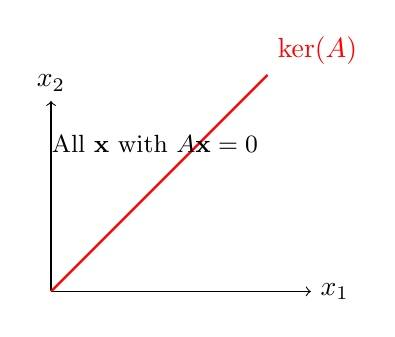
\begin{tikzpicture}[scale=1.1]
        % Axes
        \draw[->] (0,0) -- (3,0) node[right] {\(x_1\)};
        \draw[->] (0,0) -- (0,2.2) node[above] {\(x_2\)};
        % Null space line
        \draw[thick,red] (0,0) -- (2.5,2.5) node[above right] {\(\ker(A)\)};
        % Label
        \node at (1.2,1.7) {\small All \(\mathbf{x}\) with \(A\mathbf{x}=0\)};
    \end{tikzpicture}
    \caption{The null space consists of all solutions to \(A\mathbf{x}=0\).}
\end{figure}

\begin{theorem}{Fundamental Theorem of Linear Algebra}{ftla}
    For any \(A\in\mathbb{R}^{m\times n}\):
    \begin{itemize}[nosep]
        \item The column space and null space are subspaces of \(\mathbb{R}^m\) and \(\mathbb{R}^n\), respectively.
        \item The row space and left null space (null space of \(A^T\)) are subspaces of \(\mathbb{R}^n\) and \(\mathbb{R}^m\), respectively.
        \item \textbf{Rank-nullity theorem:}
              \[
                  \operatorname{rank}(A) + \operatorname{nullity}(A) = n.
              \]
    \end{itemize}
\end{theorem}

\begin{table}[H]
    \centering
    \renewcommand{\arraystretch}{1.2}
    \begin{tabular}{l|l|l}
        \textbf{Subspace} & \textbf{Definition}                & \textbf{Dimension}            \\
        \hline
        Column space      & \(\{\mathbf{y} = A\mathbf{x}\}\)   & \(\operatorname{rank}(A)\)    \\
        Row space         & \(\{\mathbf{z} = \mathbf{y}A\}\)   & \(\operatorname{rank}(A)\)    \\
        Null space        & \(\{\mathbf{x} : A\mathbf{x}=0\}\) & \(\operatorname{nullity}(A)\) \\
        Left null space   & \(\{\mathbf{y} : \mathbf{y}A=0\}\) & \(m-\operatorname{rank}(A)\)  \\
    \end{tabular}
    \caption{Summary of fundamental subspaces of a matrix.}
\end{table}

\subsection{Eigenvalues and Eigenvectors}

\begin{definition}{Eigenvalues and Eigenvectors}{eig}
    Let \(A \in \mathbb{R}^{n \times n}\). A scalar \(\lambda \in \mathbb{C}\) is an \emph{eigenvalue} of \(A\) if there exists a nonzero vector \(\mathbf{v} \in \mathbb{C}^n\) such that
    \[
        A\mathbf{v} = \lambda\mathbf{v}.
    \]
    The vector \(\mathbf{v}\) is called an \emph{eigenvector} of \(A\) corresponding to \(\lambda\).
\end{definition}

\begin{itemize}[nosep]
    \item The set of all eigenvalues of \(A\) is called the \emph{spectrum} of \(A\), denoted \(\sigma(A)\).
    \item The equation \(\det(A - \lambda I) = 0\) is called the \emph{characteristic equation}; its roots are the eigenvalues.
    \item The \emph{eigenspace} for \(\lambda\) is \(\ker(A - \lambda I)\), the set of all eigenvectors (plus \(\mathbf{0}\)) for \(\lambda\).
    \item The \emph{algebraic multiplicity} of \(\lambda\) is its multiplicity as a root of the characteristic polynomial.
    \item The \emph{geometric multiplicity} of \(\lambda\) is \(\dim\ker(A - \lambda I)\).
\end{itemize}

\begin{remark}{Geometric Interpretation}{eig-geom}
    An eigenvector \(\mathbf{v}\) is a direction that is only stretched or shrunk (by \(\lambda\)) by \(A\), not rotated. If \(A\) is real but has complex eigenvalues, the action involves rotation and scaling in a plane.
\end{remark}

\begin{example}{Eigenvalues and Eigenvectors of a \(2\times2\) Matrix}{eig-2x2}
    Let
    \[
        A = \begin{pmatrix}
            2 & 1 \\
            1 & 2
        \end{pmatrix}.
    \]
    The characteristic polynomial is
    \[
        \det(A - \lambda I) = (2-\lambda)^2 - 1 = \lambda^2 - 4\lambda + 3 = (\lambda-3)(\lambda-1).
    \]
    Thus, the eigenvalues are \(\lambda_1 = 3\) and \(\lambda_2 = 1\).
    For \(\lambda_1 = 3\):
    \[
        (A - 3I)\mathbf{v} = 0 \implies
        \begin{pmatrix}
            -1 & 1  \\
            1  & -1
        \end{pmatrix}
        \begin{pmatrix}
            v_1 \\ v_2
        \end{pmatrix}
        = 0,
    \]
    so \(v_1 = v_2\). Any nonzero multiple of \(\begin{pmatrix}1\\1\end{pmatrix}\) is an eigenvector for \(\lambda=3\).
    For \(\lambda_2 = 1\):
    \[
        (A - I)\mathbf{v} = 0 \implies
        \begin{pmatrix}
            1 & 1 \\
            1 & 1
        \end{pmatrix}
        \begin{pmatrix}
            v_1 \\ v_2
        \end{pmatrix}
        = 0,
    \]
    so \(v_1 = -v_2\). Any nonzero multiple of \(\begin{pmatrix}1\\-1\end{pmatrix}\) is an eigenvector for \(\lambda=1\).
\end{example}

\begin{remark}{Diagonalization}{eig-diag}
    If \(A\) has \(n\) linearly independent eigenvectors, then \(A\) is diagonalizable: \(A = PDP^{-1}\), where \(D\) is diagonal with the eigenvalues of \(A\) and \(P\) has the eigenvectors as columns.
\end{remark}

\subsection{Jordan Canonical Form}

\begin{definition}{Jordan Canonical Form}{jordan-form}
    Let \(A \in \mathbb{C}^{n \times n}\). The \emph{Jordan canonical form} (or \emph{Jordan normal form}) of \(A\) is a block-diagonal matrix \(J\) such that
    \[
        A = PJP^{-1}
    \]
    for some invertible matrix \(P\), where \(J\) is composed of \emph{Jordan blocks} along the diagonal. Each Jordan block \(J_k(\lambda)\) associated with eigenvalue \(\lambda\) is of the form
    \[
        J_k(\lambda) =
        \begin{pmatrix}
            \lambda & 1       &        &         & 0       \\
            0       & \lambda & 1      &         &         \\
            \vdots  & \ddots  & \ddots & \ddots  &         \\
            0       & \cdots  & 0      & \lambda & 1       \\
            0       & \cdots  & \cdots & 0       & \lambda
        \end{pmatrix}
        \in \mathbb{C}^{k \times k}
    \]
    where \(\lambda\) is on the diagonal, \(1\)'s are on the superdiagonal, and \(0\) elsewhere.
\end{definition}

\subsubsection{Existence and Uniqueness of Jordan Form}

For any square matrix \(A \in \mathbb{C}^{n \times n}\), there exists an invertible matrix \(P\) such that
\[
    A = PJP^{-1},
\]
where \(J\) is in Jordan canonical form. The Jordan form \(J\) is unique up to the ordering of its Jordan blocks; that is, the sizes and number of blocks associated with each eigenvalue are uniquely determined by \(A\).

The Jordan canonical form generalizes diagonalization: \(A\) is diagonalizable if and only if all Jordan blocks are \(1 \times 1\). Larger blocks indicate the presence of generalized eigenvectors and the failure of diagonalizability.

\begin{remark}{Intuition and Geometric Meaning}{jordan-intuition-geometry}
    The Jordan form captures the structure of \(A\) in terms of its eigenvalues and generalized eigenvectors.
    \medskip
    Each Jordan block corresponds to an eigenvalue \(\lambda\) and describes how \(A\) acts on the space spanned by its eigenvectors and generalized eigenvectors.
    \begin{itemize}[nosep]
        \item If \(A\) is diagonalizable, it stretches vectors along independent directions (eigenvectors).
        \item If not, the superdiagonal \(1\)'s in a Jordan block represent a "shear" in addition to scaling.
        \item The size of the Jordan blocks (the number of \(1\)'s on the superdiagonal) shows how many generalized eigenvectors are needed to fully describe the action of \(A\).
    \end{itemize}
\end{remark}
\begin{example}{Jordan Block Chain of Generalized Eigenvectors}{jordan-block-chain}
    For a Jordan block of size \(k\) for eigenvalue \(\lambda\), there is a chain \(\{\mathbf{v}_1, \dots, \mathbf{v}_k\}\) with

    \[
        (A - \lambda I)\mathbf{v}_1 = 0, \quad (A - \lambda I)\mathbf{v}_j = \mathbf{v}_{j-1} \ (j \geq 2).
    \]

    Here, \(\mathbf{v}_1\) is an eigenvector, and each \(\mathbf{v}_j\) (\(j>1\)) is a generalized eigenvector. \(A\) acts by scaling on \(\mathbf{v}_1\), and by scaling plus a shift (shear) along the chain for \(\mathbf{v}_j\).
    \begin{figure}[H]
        \centering
        \begin{tikzpicture}[scale=1.2]
            \draw[->,thick] (-0.2,0) -- (2.7,0) node[right] {\(x\)};
            \draw[->,thick] (0,-0.2) -- (0,2.2) node[above] {\(y\)};
            \draw[->,thick,thm-color] (0,0) -- (1.2,0.8) node[above left=2pt] {\(\mathbf{v}_1\)};
            \draw[->,thick,thm-color!60!black!80!white,dashed] (0,0) -- (0.6,1.6) node[left=2pt] {\(\mathbf{v}_2\)};
            \draw[->,thick,red] (0,0) -- (2.4,1.6) node[above right=2pt] {\(A\mathbf{v}_1\)};
            \draw[->,thick,red,dashed] (0,0) -- (1.8,3.2) node[right=2pt] {\(A\mathbf{v}_2\)};
            \fill[thm-color] (1.2,0.8) circle (1.2pt);
            \fill[thm-color!60!black!80!white] (0.6,1.6) circle (1.2pt);
            \fill[red] (2.4,1.6) circle (1.2pt);
            \fill[red] (1.8,3.2) circle (1.2pt);
            \begin{scope}[shift={(2.2,0.5)}]
                \draw[thm-color,thick] (0,0) -- (0.5,0) node[right,black] {\small \(\mathbf{v}_1\)};
                \draw[thm-color!60!black!80!white,thick,dashed] (0,-0.3) -- (0.5,-0.3) node[right,black] {\small \(\mathbf{v}_2\)};
                \draw[red,thick] (0,-0.6) -- (0.5,-0.6) node[right,black] {\small \(A\mathbf{v}_1\)};
                \draw[red,thick,dashed] (0,-0.9) -- (0.5,-0.9) node[right,black] {\small \(A\mathbf{v}_2\)};
            \end{scope}
        \end{tikzpicture}
        \caption{Jordan block: \(A\mathbf{v}_1 = \lambda\mathbf{v}_1\), \(A\mathbf{v}_2 = \lambda\mathbf{v}_2 + \mathbf{v}_1\).}
    \end{figure}
\end{example}


\subsubsection{Generalized Eigenvectors and Chains}
A \emph{generalized eigenvector} \(\mathbf{v}\) of \(A\) for eigenvalue \(\lambda\) satisfies
\[
    (A-\lambda I)^k \mathbf{v} = 0
\]
for some \(k \geq 1\). The smallest such \(k\) is called the \emph{length of the chain}. The set of all generalized eigenvectors for \(\lambda\) forms the \emph{generalized eigenspace}:
\[
    \mathcal{G}_\lambda = \left\{ \mathbf{v} \in \mathbb{C}^n : (A-\lambda I)^m \mathbf{v} = 0 \text{ for some } m \geq 1 \right\}.
\]

\begin{example}{Generalized Eigenvector Chain}
    Let
    \[
        A = \begin{pmatrix}
            2 & 1 & 0 \\
            0 & 2 & 1 \\
            0 & 0 & 2
        \end{pmatrix}.
    \]
    The only eigenvalue is \(\lambda=2\). The vector \(\mathbf{v}_1 = \begin{pmatrix}1\\0\\0\end{pmatrix}\) is an eigenvector:
    \[
        (A-2I)\mathbf{v}_1 = 0.
    \]
    Now, \(\mathbf{v}_2 = \begin{pmatrix}0\\1\\0\end{pmatrix}\) is a generalized eigenvector of order \(2\):
    \[
        (A-2I)\mathbf{v}_2 = \begin{pmatrix}0\\0\\0\end{pmatrix} \neq 0, \quad (A-2I)^2\mathbf{v}_2 = 0.
    \]
    Similarly, \(\mathbf{v}_3 = \begin{pmatrix}0\\0\\1\end{pmatrix}\) is a generalized eigenvector of order \(3\):
    \[
        (A-2I)\mathbf{v}_3 = \mathbf{v}_2, \quad (A-2I)^2\mathbf{v}_3 = \mathbf{v}_1, \quad (A-2I)^3\mathbf{v}_3 = 0.
    \]
    Thus, \(\{\mathbf{v}_1, \mathbf{v}_2, \mathbf{v}_3\}\) forms a chain of generalized eigenvectors for \(\lambda=2\).
\end{example}

\subsubsection{Structure of Jordan Form}
For each eigenvalue \(\lambda\):
\begin{itemize}[nosep]
    \item The number of Jordan blocks equals the geometric multiplicity (dimension of \(\ker(A-\lambda I)\)).
    \item The sum of the sizes of the Jordan blocks equals the algebraic multiplicity (multiplicity of \(\lambda\) as a root of the characteristic polynomial).
\end{itemize}

\begin{example}{Jordan Form Example}{jordan-example}
    Suppose \(A\) has characteristic polynomial \((x-2)^3\) but only one linearly independent eigenvector for \(\lambda=2\). Then
    \[
        J =
        \begin{pmatrix}
            2 & 1 & 0 \\
            0 & 2 & 1 \\
            0 & 0 & 2
        \end{pmatrix}
    \]
    is the Jordan form: a single \(3 \times 3\) block for \(\lambda=2\).
\end{example}

\emph{Why Jordan Form Matters}

\begin{itemize}[nosep]
    \item It provides a complete classification of matrices up to similarity.
    \item It is essential for understanding the behavior of \(A^k\), \(\exp(A)\), and solutions to differential equations \(\dot{\mathbf{x}} = A\mathbf{x}\).
    \item It reveals the "obstructions" to diagonalization: the off-diagonal \(1\)'s indicate nontrivial chains of generalized eigenvectors.
\end{itemize}

\begin{remark}{Real Matrices}{jordan-real}
    Every real matrix has a Jordan form over \(\mathbb{C}\). Over \(\mathbb{R}\), the canonical form may involve \(2 \times 2\) blocks for complex conjugate eigenvalues.
\end{remark}

\subsection{Matrix and Vector Norms}
Norms formalize the notion of size or length for vectors and matrices, providing a way to measure distances and magnitudes in linear algebra.
\begin{definition}{Vector Norm}{vector-norm}
    A \emph{norm} on \(\mathbb{R}^n\) is a function \(\lVert \cdot \rVert : \mathbb{R}^n \to [0, \infty)\) such that, for all \(\mathbf{x}, \mathbf{y} \in \mathbb{R}^n\) and \(\alpha \in \mathbb{R}\):
    \begin{enumerate}[nosep]
        \item \textbf{Definiteness:} \(\lVert \mathbf{x} \rVert = 0 \iff \mathbf{x} = \mathbf{0}\)
        \item \textbf{Homogeneity:} \(\lVert \alpha \mathbf{x} \rVert = |\alpha| \lVert \mathbf{x} \rVert\)
        \item \textbf{Triangle inequality:} \(\lVert \mathbf{x} + \mathbf{y} \rVert \leq \lVert \mathbf{x} \rVert + \lVert \mathbf{y} \rVert\)
    \end{enumerate}
    \medskip
    \noindent
    \textbf{Common norms for} \(\mathbf{x} = (x_1, \dots, x_n)^\top\):
    \begin{align*}
        \text{\(p\)-norm:} \qquad     & \lVert \mathbf{x} \rVert_p = \left( \sum_{i=1}^n |x_i|^p \right)^{1/p}, \quad 1 \leq p < \infty \\[0.5em]
        \text{Infinity norm:} \qquad  & \lVert \mathbf{x} \rVert_\infty = \max_{1 \leq i \leq n} |x_i|                                  \\[0.5em]
        \text{Euclidean norm:} \qquad & \lVert \mathbf{x} \rVert_2 = \left( \sum_{i=1}^n |x_i|^2 \right)^{1/2}
    \end{align*}
\end{definition}

\begin{definition}{Matrix Norm}{matrix-norm}
    A \emph{matrix norm} \(\lVert \cdot \rVert\) on \(\mathbb{R}^{m \times n}\) is a function \(\lVert \cdot \rVert : \mathbb{R}^{m \times n} \to [0, \infty)\) satisfying properties analogous to vector norms.

    \medskip
    \noindent
    An \emph{induced} (operator) norm, subordinate to a vector norm \(\lVert \cdot \rVert\), is defined by
    \[
        \lVert A \rVert = \sup_{\mathbf{x} \neq \mathbf{0}} \frac{\lVert A\mathbf{x} \rVert}{\lVert \mathbf{x} \rVert} = \sup_{\lVert \mathbf{x} \rVert = 1} \lVert A\mathbf{x} \rVert.
    \]
    \medskip
    \noindent
    \textbf{Common induced norms for} \(A = (a_{ij}) \in \mathbb{R}^{m \times n}\):
    \begin{align*}
        \text{1-norm:} \qquad                 & \lVert A \rVert_1 = \max_{1 \leq j \leq n} \sum_{i=1}^m |a_{ij}| \quad \text{(maximum column sum)}                      \\[0.5em]
        \text{Infinity norm:} \qquad          & \lVert A \rVert_\infty = \max_{1 \leq i \leq m} \sum_{j=1}^n |a_{ij}| \quad \text{(maximum row sum)}                    \\[0.5em]
        \text{2-norm (spectral norm):} \qquad & \lVert A \rVert_2 = \sup_{\lVert \mathbf{x} \rVert_2 = 1} \lVert A\mathbf{x} \rVert_2 = \sqrt{\lambda_{\max}(A^\top A)}
    \end{align*}
    where \(\lambda_{\max}(A^\top A)\) denotes the largest eigenvalue of \(A^\top A\).
\end{definition}

\subsection{Spectral Radius}
The spectral radius of a matrix measures the largest \enquote{scaling} by which the matrix can stretch a vector, as determined by its eigenvalues.

\begin{definition}{Spectral Radius}{spectral-radius}
    The \emph{spectral radius} of a square matrix \(A \in \mathbb{R}^{n \times n}\) is the largest modulus among its eigenvalues:
    \[
        \rho(A) = \max \left\{ |\lambda| : \lambda \in \sigma(A) \right\},
    \]
    where \(\sigma(A)\) denotes the set of all eigenvalues of \(A\). That is, if \(A\) has eigenvalues \(\lambda_1, \lambda_2, \dots, \lambda_n\), then
    \[
        \rho(A) = \max_{1 \leq i \leq n} |\lambda_i|.
    \]
\end{definition}
Intuitively, it describes the long-term behavior of repeated matrix multiplication: if the spectral radius is less than one, powers of the matrix tend to zero; if greater than one, they grow without bound.
\subsection{Condition Number}

The condition number of a matrix measures how sensitive the solution of \(A\mathbf{x} = \mathbf{b}\) is to small changes in \(A\) or \(\mathbf{b}\). A large condition number indicates that the system is \emph{ill-conditioned}: small errors in the data can cause large errors in the solution. If the condition number is close to \(1\), the system is \emph{well-conditioned}.
\begin{definition}{Condition Number}{cond-num}
    Let \(A \in \mathbb{R}^{n \times n}\) be an invertible matrix, and let \(\lVert \cdot \rVert\) be a matrix norm. The \emph{condition number} of \(A\) with respect to \(\lVert \cdot \rVert\) is defined as:
    \[
        \kappa(A) = \lVert A \rVert \cdot \lVert A^{-1} \rVert.
    \]
\end{definition}

\begin{property}{Condition Number and Singular Values}{cond-num-singular}
    The condition number varies with the matrix norm used:
    \begin{align*}
        \text{\(2\)-norm:} \qquad & \kappa_2(A) = \frac{\sigma_{\max}(A)}{\sigma_{\min}(A)} \\
        \text{\(1\)-norm:} \qquad & \kappa_1(A) = \lVert A \rVert_1 \cdot \lVert A^{-1} \rVert_1 \\
        \text{\(\infty\)-norm:} \qquad & \kappa_\infty(A) = \lVert A \rVert_\infty \cdot \lVert A^{-1} \rVert_\infty
    \end{align*}
    where \(\sigma_{\max}(A)\) and \(\sigma_{\min}(A)\) denote the largest and smallest singular values of \(A\), respectively.
\end{property}

\begin{remark}{Condition Number for Symmetric Positive Definite Matrices}{cond-num-symmetric}
    If \(A \in \mathbb{R}^{n \times n}\) is symmetric positive definite, the singular values of \(A\) are equal to the absolute values of its eigenvalues. Thus, the condition number in the \(2\)-norm simplifies to:
    \[
        \kappa_2(A) = \frac{\lambda_{\max}(A)}{\lambda_{\min}(A)},
    \]
    where \(\lambda_{\max}(A)\) and \(\lambda_{\min}(A)\) are the largest and smallest eigenvalues of \(A\), respectively.
\end{remark}

\begin{remark}{Geometric Interpretation of Condition Number}{cond-num-geometry}
    The condition number describes how much \(A\) stretches the unit sphere into an ellipsoid. A large condition number indicates that the ellipsoid is highly elongated, meaning some directions are stretched significantly more than others. This implies that the matrix \(A\) is \emph{ill-conditioned}, and small perturbations in the input can lead to large changes in the output.
\end{remark}

\begin{figure}[H]
    \centering
    \begin{tikzpicture}
        \draw[thick, spaceblack] (0,0) circle (1);
        \draw[red, thick, dashed, rotate=10] (0,0) ellipse (2.2 and 0.5);
        \draw[green!70!black,dashed, thick] (0,0) ellipse (1.1 and 0.9);
        \begin{scope}[shift={(3.2,0.7)}]
            \draw[spaceblack,thick] (0,0) -- (0.7,0) node[right,black] {\small Unit circle};
            \draw[red, thick, dashed] (0,-0.4) -- (0.7,-0.4) node[right,black] {\small \(A\) (ill-conditioned)};
            \draw[green!70!black, thick, dashed] (0,-0.8) -- (0.7,-0.8) node[right,black] {\small \(A\) (well-conditioned)};
        \end{scope}
    \end{tikzpicture}
    \caption{Effect of \(A\) on the unit circle: well-conditioned (nearly circular) vs. ill-conditioned (stretched).}
\end{figure}

\begin{figure}[H]
    \centering
    \begin{tikzpicture}[scale=1]
        \draw[->,thick] (-0.3,0) -- (2.7,0) node[right] {\(x\)};
        \draw[->,thick] (0,-0.3) -- (0,2.1) node[above] {\(y\)};
        \draw[spaceblack, dashed, thick] (0,0) -- (2.2,1.85);
        \draw[->,thick,thm-color] (0,0) -- (1.1,0.925) node[above left=2pt] {\(\mathbf{v}\)};
        \draw[->,thick,red] (0,0) -- (2.2,1.85) node[above right=2pt] {\(A\mathbf{v} = \lambda\mathbf{v}\)};
        \fill[thm-color] (1.1,0.925) circle (1.2pt);
        \fill[red] (2.2,1.85) circle (1.2pt);
        \node[red] at (1.65,1.4) {\small \(\lambda > 1\)};
    \end{tikzpicture}
    \caption{An eigenvector \(\mathbf{v}\) is only stretched (not rotated) by \(A\): \(A\mathbf{v} = \lambda\mathbf{v}\)}
\end{figure}


\section{Complex Numbers and Fields}
\label{sec:complex-fields}

\subsection{Complex Numbers}

\begin{definition}{Complex Numbers}{complex-numbers}
    The set of complex numbers is
    \[
        \mathbb{C} = \{ z = x + iy : x, y \in \mathbb{R},\ i^2 = -1 \}.
    \]
    The real part is \(\Re(z) = x\), the imaginary part is \(\Im(z) = y\), and the complex conjugate is \(\overline{z} = x - iy\).
\end{definition}

\begin{remark}{Connection to Linear Algebra}{complex-linalg}
    Complex numbers extend the field of real numbers, allowing us to define vector spaces and matrices over \(\mathbb{C}\) as well as \(\mathbb{R}\). Many linear algebra concepts, such as eigenvalues and diagonalization, naturally generalize to complex vector spaces.
\end{remark}

\begin{property}{Modulus and Argument}{modulus-argument}
    The modulus of \(z\) is \(|z| = \sqrt{x^2 + y^2}\). The argument is \(\arg(z) = \arctan2(y, x)\).
    Euler's formula: \(z = r e^{i\theta}\), where \(r = |z|\), \(\theta = \arg(z)\).
\end{property}

\subsection{Fields}

\begin{definition}{Field}{field}
    A \emph{field} \(\mathbb{K}\) is a set with two operations, addition and multiplication, such that:
    \begin{itemize}[nosep]
        \item \((\mathbb{K}, +)\) is an abelian group with identity \(0\).
        \item \((\mathbb{K} \setminus \{0\}, \cdot)\) is an abelian group with identity \(1\).
        \item Multiplication is distributive over addition.
    \end{itemize}
    Examples: \(\mathbb{R}\), \(\mathbb{C}\), \(\mathbb{Q}\).
\end{definition}

\begin{remark}{Fields in Linear Algebra}{fields-linalg}
    Linear algebra is built on the concept of vector spaces over a field. The choice of field (e.g., \(\mathbb{R}\) or \(\mathbb{C}\)) determines the properties of the vector spaces and matrices we study.
\end{remark}

\section{Polynomials}
\label{sec:polynomials}

\begin{definition}{Polynomial}{polynomial}
    A polynomial of degree \(n\) over a field \(\mathbb{K}\) is
    \[
        p(x) = a_0 + a_1 x + \cdots + a_n x^n, \quad a_n \neq 0,\ a_i \in \mathbb{K}.
    \]
\end{definition}

\begin{property}{Roots and Factorization}{roots-factorization}
    A polynomial of degree \(n\) has at most \(n\) roots in \(\mathbb{K}\). Over \(\mathbb{C}\), every polynomial of degree \(n\) has exactly \(n\) roots (counting multiplicities).
\end{property}

\begin{definition}{Multiplicity of a Root}{root-multiplicity}
    The root \(r\) of \(p(x)\) has multiplicity \(k\) if \((x - r)^k\) divides \(p(x)\), but \((x - r)^{k+1}\) does not.
\end{definition}

\section{Systems of Linear Equations}

\subsection{Solving Linear Systems}

\begin{definition}{Linear System}{linear-system}
    A system of \(m\) linear equations in \(n\) variables:
    \[
        A\mathbf{x} = \mathbf{b}, \quad A \in \mathbb{R}^{m \times n},\ \mathbf{x} \in \mathbb{R}^n,\ \mathbf{b} \in \mathbb{R}^m.
    \]
\end{definition}

\begin{itemize}[nosep]
    \item If \(A\) is square and invertible, the unique solution is \(\mathbf{x} = A^{-1}\mathbf{b}\).
    \item If \(A\) is not invertible or not square, solutions may not exist or may not be unique.
\end{itemize}

\subsection{Gaussian Elimination}

\begin{definition}{Gaussian Elimination}{gauss-elim}
    A systematic procedure to solve \(A\mathbf{x} = \mathbf{b}\) by reducing \(A\) to row echelon form using elementary row operations.
\end{definition}

\begin{remark}{Pivoting}{pivoting}
    Pivoting (row exchanges) is used to avoid division by zero and reduce numerical errors.
\end{remark}

\section{Basic Set Theory and Functions}

\subsection{Sets and Mappings}

\begin{definition}{Set}{set}
    A set is a collection of distinct objects. Notation: \(A = \{a_1, a_2, \ldots\}\).
\end{definition}

\begin{definition}{Function (Mapping)}{function}
    A function \(f : X \to Y\) assigns to each \(x \in X\) a unique \(y = f(x) \in Y\).
\end{definition}

\begin{itemize}[nosep]
    \item \(f\) is injective (one-to-one) if \(f(x_1) = f(x_2) \implies x_1 = x_2\).
    \item \(f\) is surjective (onto) if for every \(y \in Y\), there exists \(x \in X\) with \(f(x) = y\).
    \item \(f\) is bijective if it is both injective and surjective.
\end{itemize}

\section{Basic Topology in \texorpdfstring{$\mathbb{R}^n$}{Rn}}

\subsection{Open and Closed Sets}

\begin{definition}{Open Set}{open-set}
    A set \(U \subset \mathbb{R}^n\) is open if for every \(x \in U\), there exists \(\varepsilon > 0\) such that the ball \(B(x, \varepsilon) \subset U\).
\end{definition}

\begin{definition}{Closed Set}{closed-set}
    A set \(F \subset \mathbb{R}^n\) is closed if its complement is open, or equivalently, if it contains all its limit points.
\end{definition}

\subsection{Boundedness and Compactness}

\begin{definition}{Bounded Set}{bounded-set}
    \(S \subset \mathbb{R}^n\) is bounded if there exists \(M > 0\) such that \(\lVert x \rVert < M\) for all \(x \in S\).
\end{definition}

\begin{definition}{Compact Set}{compact-set}
    \(K \subset \mathbb{R}^n\) is compact if it is closed and bounded (Heine-Borel theorem).
\end{definition}

\section{Sequences and Limits}

\begin{definition}{Sequence}{sequence}
    A sequence in \(\mathbb{R}^n\) is a function \(x : \mathbb{N} \to \mathbb{R}^n\), written as \((x_k)\).
\end{definition}

\begin{definition}{Limit of a Sequence}{sequence-limit}
    \((x_k)\) converges to \(x\) if for every \(\varepsilon > 0\), there exists \(N\) such that \(k \geq N \implies \lVert x_k - x \rVert < \varepsilon\).
\end{definition}

\section{Basic Calculus in Several Variables}

\subsection{Continuity and Differentiability}

\begin{definition}{Continuous Function}{continuous}
    \(f : \mathbb{R}^n \to \mathbb{R}^m\) is continuous at \(x_0\) if for every \(\varepsilon > 0\), there exists \(\delta > 0\) such that \(\lVert x - x_0 \rVert < \delta \implies \lVert f(x) - f(x_0) \rVert < \varepsilon\).
\end{definition}

\begin{definition}{Differentiable Function}{differentiable}
    \(f : \mathbb{R}^n \to \mathbb{R}^m\) is differentiable at \(x_0\) if there exists a linear map \(A : \mathbb{R}^n \to \mathbb{R}^m\) such that
    \[
        \lim_{h \to 0} \frac{\lVert f(x_0 + h) - f(x_0) - A h \rVert}{\lVert h \rVert} = 0.
    \]
    The matrix \(A\) is the Jacobian of \(f\) at \(x_0\).
\end{definition}

\section{Basic Notation and Conventions}

\begin{itemize}[nosep]
    \item \(\mathbb{N}\): natural numbers, \(\mathbb{Z}\): integers, \(\mathbb{Q}\): rationals, \(\mathbb{R}\): reals, \(\mathbb{C}\): complex numbers.
    \item Vectors are columns by default; \(\mathbf{x}\) denotes a vector, \(A\) a matrix.
    \item \(\lVert \cdot \rVert\) denotes a norm; \(\langle \cdot, \cdot \rangle\) denotes an inner product.
    \item \(I_n\): \(n \times n\) identity matrix; \(0\): zero vector or matrix (context-dependent).
\end{itemize}